% Created by tikzDevice version 0.11 on 2018-09-10 16:39:11
% !TEX encoding = UTF-8 Unicode
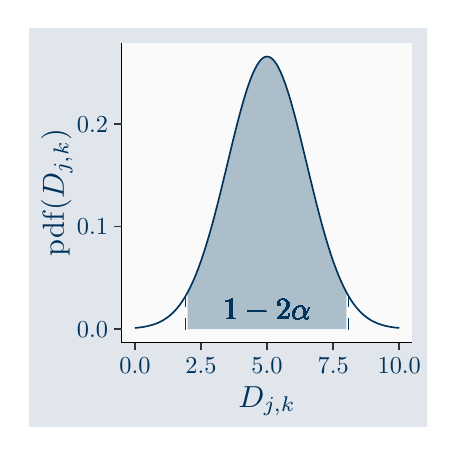
\begin{tikzpicture}[x=1pt,y=1pt]
\definecolor{fillColor}{RGB}{255,255,255}
\path[use as bounding box,fill=fillColor,fill opacity=0.00] (0,0) rectangle (144.54,144.54);
\begin{scope}
\path[clip] (  0.00,  0.00) rectangle (144.54,144.54);
\definecolor{drawColor}{RGB}{255,255,255}
\definecolor{fillColor}{RGB}{225,229,236}

\path[draw=drawColor,line width= 0.6pt,line join=round,line cap=round,fill=fillColor] (  0.00, -0.00) rectangle (144.54,144.54);
\end{scope}
\begin{scope}
\path[clip] ( 33.96, 30.72) rectangle (139.04,139.04);
\definecolor{fillColor}{gray}{0.98}

\path[fill=fillColor] ( 33.96, 30.72) rectangle (139.04,139.04);
\definecolor{fillColor}{RGB}{173,190,203}

\path[fill=fillColor] ( 57.84, 48.97) --
	( 58.80, 50.84) --
	( 59.75, 52.89) --
	( 60.71, 55.13) --
	( 61.66, 57.57) --
	( 62.62, 60.20) --
	( 63.57, 63.03) --
	( 64.53, 66.04) --
	( 65.49, 69.24) --
	( 66.44, 72.60) --
	( 67.40, 76.13) --
	( 68.35, 79.79) --
	( 69.31, 83.58) --
	( 70.26, 87.45) --
	( 71.22, 91.40) --
	( 72.17, 95.37) --
	( 73.13, 99.35) --
	( 74.08,103.29) --
	( 75.04,107.15) --
	( 75.99,110.90) --
	( 76.95,114.50) --
	( 77.90,117.90) --
	( 78.86,121.06) --
	( 79.81,123.96) --
	( 80.77,126.55) --
	( 81.72,128.80) --
	( 82.68,130.68) --
	( 83.64,132.17) --
	( 84.59,133.25) --
	( 85.55,133.90) --
	( 86.50,134.12) --
	( 87.46,133.90) --
	( 88.41,133.25) --
	( 89.37,132.17) --
	( 90.32,130.68) --
	( 91.28,128.80) --
	( 92.23,126.55) --
	( 93.19,123.96) --
	( 94.14,121.06) --
	( 95.10,117.90) --
	( 96.05,114.50) --
	( 97.01,110.90) --
	( 97.96,107.15) --
	( 98.92,103.29) --
	( 99.87, 99.35) --
	(100.83, 95.37) --
	(101.78, 91.40) --
	(102.74, 87.45) --
	(103.70, 83.58) --
	(104.65, 79.79) --
	(105.61, 76.13) --
	(106.56, 72.60) --
	(107.52, 69.24) --
	(108.47, 66.04) --
	(109.43, 63.03) --
	(110.38, 60.20) --
	(111.34, 57.57) --
	(112.29, 55.13) --
	(113.25, 52.89) --
	(114.20, 50.84) --
	(115.16, 48.97) --
	(115.16, 35.65) --
	(114.20, 35.65) --
	(113.25, 35.65) --
	(112.29, 35.65) --
	(111.34, 35.65) --
	(110.38, 35.65) --
	(109.43, 35.65) --
	(108.47, 35.65) --
	(107.52, 35.65) --
	(106.56, 35.65) --
	(105.61, 35.65) --
	(104.65, 35.65) --
	(103.70, 35.65) --
	(102.74, 35.65) --
	(101.78, 35.65) --
	(100.83, 35.65) --
	( 99.87, 35.65) --
	( 98.92, 35.65) --
	( 97.96, 35.65) --
	( 97.01, 35.65) --
	( 96.05, 35.65) --
	( 95.10, 35.65) --
	( 94.14, 35.65) --
	( 93.19, 35.65) --
	( 92.23, 35.65) --
	( 91.28, 35.65) --
	( 90.32, 35.65) --
	( 89.37, 35.65) --
	( 88.41, 35.65) --
	( 87.46, 35.65) --
	( 86.50, 35.65) --
	( 85.55, 35.65) --
	( 84.59, 35.65) --
	( 83.64, 35.65) --
	( 82.68, 35.65) --
	( 81.72, 35.65) --
	( 80.77, 35.65) --
	( 79.81, 35.65) --
	( 78.86, 35.65) --
	( 77.90, 35.65) --
	( 76.95, 35.65) --
	( 75.99, 35.65) --
	( 75.04, 35.65) --
	( 74.08, 35.65) --
	( 73.13, 35.65) --
	( 72.17, 35.65) --
	( 71.22, 35.65) --
	( 70.26, 35.65) --
	( 69.31, 35.65) --
	( 68.35, 35.65) --
	( 67.40, 35.65) --
	( 66.44, 35.65) --
	( 65.49, 35.65) --
	( 64.53, 35.65) --
	( 63.57, 35.65) --
	( 62.62, 35.65) --
	( 61.66, 35.65) --
	( 60.71, 35.65) --
	( 59.75, 35.65) --
	( 58.80, 35.65) --
	( 57.84, 35.65) --
	cycle;
\definecolor{drawColor}{RGB}{0,52,92}

\path[draw=drawColor,line width= 0.6pt,line join=round] ( 38.74, 36.03) --
	( 39.69, 36.12) --
	( 40.65, 36.24) --
	( 41.60, 36.37) --
	( 42.56, 36.54) --
	( 43.51, 36.74) --
	( 44.47, 36.98) --
	( 45.42, 37.27) --
	( 46.38, 37.60) --
	( 47.34, 38.00) --
	( 48.29, 38.46) --
	( 49.25, 39.00) --
	( 50.20, 39.63) --
	( 51.16, 40.35) --
	( 52.11, 41.18) --
	( 53.07, 42.12) --
	( 54.02, 43.19) --
	( 54.98, 44.40) --
	( 55.93, 45.76) --
	( 56.89, 47.29) --
	( 57.84, 48.97) --
	( 58.80, 50.84) --
	( 59.75, 52.89) --
	( 60.71, 55.13) --
	( 61.66, 57.57) --
	( 62.62, 60.20) --
	( 63.57, 63.03) --
	( 64.53, 66.04) --
	( 65.49, 69.24) --
	( 66.44, 72.60) --
	( 67.40, 76.13) --
	( 68.35, 79.79) --
	( 69.31, 83.58) --
	( 70.26, 87.45) --
	( 71.22, 91.40) --
	( 72.17, 95.37) --
	( 73.13, 99.35) --
	( 74.08,103.29) --
	( 75.04,107.15) --
	( 75.99,110.90) --
	( 76.95,114.50) --
	( 77.90,117.90) --
	( 78.86,121.06) --
	( 79.81,123.96) --
	( 80.77,126.55) --
	( 81.72,128.80) --
	( 82.68,130.68) --
	( 83.64,132.17) --
	( 84.59,133.25) --
	( 85.55,133.90) --
	( 86.50,134.12) --
	( 87.46,133.90) --
	( 88.41,133.25) --
	( 89.37,132.17) --
	( 90.32,130.68) --
	( 91.28,128.80) --
	( 92.23,126.55) --
	( 93.19,123.96) --
	( 94.14,121.06) --
	( 95.10,117.90) --
	( 96.05,114.50) --
	( 97.01,110.90) --
	( 97.96,107.15) --
	( 98.92,103.29) --
	( 99.87, 99.35) --
	(100.83, 95.37) --
	(101.78, 91.40) --
	(102.74, 87.45) --
	(103.70, 83.58) --
	(104.65, 79.79) --
	(105.61, 76.13) --
	(106.56, 72.60) --
	(107.52, 69.24) --
	(108.47, 66.04) --
	(109.43, 63.03) --
	(110.38, 60.20) --
	(111.34, 57.57) --
	(112.29, 55.13) --
	(113.25, 52.89) --
	(114.20, 50.84) --
	(115.16, 48.97) --
	(116.11, 47.29) --
	(117.07, 45.76) --
	(118.02, 44.40) --
	(118.98, 43.19) --
	(119.93, 42.12) --
	(120.89, 41.18) --
	(121.85, 40.35) --
	(122.80, 39.63) --
	(123.76, 39.00) --
	(124.71, 38.46) --
	(125.67, 38.00) --
	(126.62, 37.60) --
	(127.58, 37.27) --
	(128.53, 36.98) --
	(129.49, 36.74) --
	(130.44, 36.54) --
	(131.40, 36.37) --
	(132.35, 36.24) --
	(133.31, 36.12) --
	(134.26, 36.03);

\path[draw=drawColor,line width= 0.6pt,dash pattern=on 4pt off 4pt ,line join=round] ( 57.07, 35.65) -- ( 57.07, 47.60);

\path[draw=drawColor,line width= 0.6pt,dash pattern=on 4pt off 4pt ,line join=round] ( 57.07, 35.65) -- ( 57.07, 47.60);

\path[draw=drawColor,line width= 0.6pt,dash pattern=on 4pt off 4pt ,line join=round] ( 57.07, 35.65) -- ( 57.07, 47.60);

\path[draw=drawColor,line width= 0.6pt,dash pattern=on 4pt off 4pt ,line join=round] ( 57.07, 35.65) -- ( 57.07, 47.60);

\path[draw=drawColor,line width= 0.6pt,dash pattern=on 4pt off 4pt ,line join=round] ( 57.07, 35.65) -- ( 57.07, 47.60);

\path[draw=drawColor,line width= 0.6pt,dash pattern=on 4pt off 4pt ,line join=round] ( 57.07, 35.65) -- ( 57.07, 47.60);

\path[draw=drawColor,line width= 0.6pt,dash pattern=on 4pt off 4pt ,line join=round] ( 57.07, 35.65) -- ( 57.07, 47.60);

\path[draw=drawColor,line width= 0.6pt,dash pattern=on 4pt off 4pt ,line join=round] ( 57.07, 35.65) -- ( 57.07, 47.60);

\path[draw=drawColor,line width= 0.6pt,dash pattern=on 4pt off 4pt ,line join=round] ( 57.07, 35.65) -- ( 57.07, 47.60);

\path[draw=drawColor,line width= 0.6pt,dash pattern=on 4pt off 4pt ,line join=round] ( 57.07, 35.65) -- ( 57.07, 47.60);

\path[draw=drawColor,line width= 0.6pt,dash pattern=on 4pt off 4pt ,line join=round] ( 57.07, 35.65) -- ( 57.07, 47.60);

\path[draw=drawColor,line width= 0.6pt,dash pattern=on 4pt off 4pt ,line join=round] ( 57.07, 35.65) -- ( 57.07, 47.60);

\path[draw=drawColor,line width= 0.6pt,dash pattern=on 4pt off 4pt ,line join=round] ( 57.07, 35.65) -- ( 57.07, 47.60);

\path[draw=drawColor,line width= 0.6pt,dash pattern=on 4pt off 4pt ,line join=round] ( 57.07, 35.65) -- ( 57.07, 47.60);

\path[draw=drawColor,line width= 0.6pt,dash pattern=on 4pt off 4pt ,line join=round] ( 57.07, 35.65) -- ( 57.07, 47.60);

\path[draw=drawColor,line width= 0.6pt,dash pattern=on 4pt off 4pt ,line join=round] ( 57.07, 35.65) -- ( 57.07, 47.60);

\path[draw=drawColor,line width= 0.6pt,dash pattern=on 4pt off 4pt ,line join=round] ( 57.07, 35.65) -- ( 57.07, 47.60);

\path[draw=drawColor,line width= 0.6pt,dash pattern=on 4pt off 4pt ,line join=round] ( 57.07, 35.65) -- ( 57.07, 47.60);

\path[draw=drawColor,line width= 0.6pt,dash pattern=on 4pt off 4pt ,line join=round] ( 57.07, 35.65) -- ( 57.07, 47.60);

\path[draw=drawColor,line width= 0.6pt,dash pattern=on 4pt off 4pt ,line join=round] ( 57.07, 35.65) -- ( 57.07, 47.60);

\path[draw=drawColor,line width= 0.6pt,dash pattern=on 4pt off 4pt ,line join=round] ( 57.07, 35.65) -- ( 57.07, 47.60);

\path[draw=drawColor,line width= 0.6pt,dash pattern=on 4pt off 4pt ,line join=round] ( 57.07, 35.65) -- ( 57.07, 47.60);

\path[draw=drawColor,line width= 0.6pt,dash pattern=on 4pt off 4pt ,line join=round] ( 57.07, 35.65) -- ( 57.07, 47.60);

\path[draw=drawColor,line width= 0.6pt,dash pattern=on 4pt off 4pt ,line join=round] ( 57.07, 35.65) -- ( 57.07, 47.60);

\path[draw=drawColor,line width= 0.6pt,dash pattern=on 4pt off 4pt ,line join=round] ( 57.07, 35.65) -- ( 57.07, 47.60);

\path[draw=drawColor,line width= 0.6pt,dash pattern=on 4pt off 4pt ,line join=round] ( 57.07, 35.65) -- ( 57.07, 47.60);

\path[draw=drawColor,line width= 0.6pt,dash pattern=on 4pt off 4pt ,line join=round] ( 57.07, 35.65) -- ( 57.07, 47.60);

\path[draw=drawColor,line width= 0.6pt,dash pattern=on 4pt off 4pt ,line join=round] ( 57.07, 35.65) -- ( 57.07, 47.60);

\path[draw=drawColor,line width= 0.6pt,dash pattern=on 4pt off 4pt ,line join=round] ( 57.07, 35.65) -- ( 57.07, 47.60);

\path[draw=drawColor,line width= 0.6pt,dash pattern=on 4pt off 4pt ,line join=round] ( 57.07, 35.65) -- ( 57.07, 47.60);

\path[draw=drawColor,line width= 0.6pt,dash pattern=on 4pt off 4pt ,line join=round] ( 57.07, 35.65) -- ( 57.07, 47.60);

\path[draw=drawColor,line width= 0.6pt,dash pattern=on 4pt off 4pt ,line join=round] ( 57.07, 35.65) -- ( 57.07, 47.60);

\path[draw=drawColor,line width= 0.6pt,dash pattern=on 4pt off 4pt ,line join=round] ( 57.07, 35.65) -- ( 57.07, 47.60);

\path[draw=drawColor,line width= 0.6pt,dash pattern=on 4pt off 4pt ,line join=round] ( 57.07, 35.65) -- ( 57.07, 47.60);

\path[draw=drawColor,line width= 0.6pt,dash pattern=on 4pt off 4pt ,line join=round] ( 57.07, 35.65) -- ( 57.07, 47.60);

\path[draw=drawColor,line width= 0.6pt,dash pattern=on 4pt off 4pt ,line join=round] ( 57.07, 35.65) -- ( 57.07, 47.60);

\path[draw=drawColor,line width= 0.6pt,dash pattern=on 4pt off 4pt ,line join=round] ( 57.07, 35.65) -- ( 57.07, 47.60);

\path[draw=drawColor,line width= 0.6pt,dash pattern=on 4pt off 4pt ,line join=round] ( 57.07, 35.65) -- ( 57.07, 47.60);

\path[draw=drawColor,line width= 0.6pt,dash pattern=on 4pt off 4pt ,line join=round] ( 57.07, 35.65) -- ( 57.07, 47.60);

\path[draw=drawColor,line width= 0.6pt,dash pattern=on 4pt off 4pt ,line join=round] ( 57.07, 35.65) -- ( 57.07, 47.60);

\path[draw=drawColor,line width= 0.6pt,dash pattern=on 4pt off 4pt ,line join=round] ( 57.07, 35.65) -- ( 57.07, 47.60);

\path[draw=drawColor,line width= 0.6pt,dash pattern=on 4pt off 4pt ,line join=round] ( 57.07, 35.65) -- ( 57.07, 47.60);

\path[draw=drawColor,line width= 0.6pt,dash pattern=on 4pt off 4pt ,line join=round] ( 57.07, 35.65) -- ( 57.07, 47.60);

\path[draw=drawColor,line width= 0.6pt,dash pattern=on 4pt off 4pt ,line join=round] ( 57.07, 35.65) -- ( 57.07, 47.60);

\path[draw=drawColor,line width= 0.6pt,dash pattern=on 4pt off 4pt ,line join=round] ( 57.07, 35.65) -- ( 57.07, 47.60);

\path[draw=drawColor,line width= 0.6pt,dash pattern=on 4pt off 4pt ,line join=round] ( 57.07, 35.65) -- ( 57.07, 47.60);

\path[draw=drawColor,line width= 0.6pt,dash pattern=on 4pt off 4pt ,line join=round] ( 57.07, 35.65) -- ( 57.07, 47.60);

\path[draw=drawColor,line width= 0.6pt,dash pattern=on 4pt off 4pt ,line join=round] ( 57.07, 35.65) -- ( 57.07, 47.60);

\path[draw=drawColor,line width= 0.6pt,dash pattern=on 4pt off 4pt ,line join=round] ( 57.07, 35.65) -- ( 57.07, 47.60);

\path[draw=drawColor,line width= 0.6pt,dash pattern=on 4pt off 4pt ,line join=round] ( 57.07, 35.65) -- ( 57.07, 47.60);

\path[draw=drawColor,line width= 0.6pt,dash pattern=on 4pt off 4pt ,line join=round] ( 57.07, 35.65) -- ( 57.07, 47.60);

\path[draw=drawColor,line width= 0.6pt,dash pattern=on 4pt off 4pt ,line join=round] ( 57.07, 35.65) -- ( 57.07, 47.60);

\path[draw=drawColor,line width= 0.6pt,dash pattern=on 4pt off 4pt ,line join=round] ( 57.07, 35.65) -- ( 57.07, 47.60);

\path[draw=drawColor,line width= 0.6pt,dash pattern=on 4pt off 4pt ,line join=round] ( 57.07, 35.65) -- ( 57.07, 47.60);

\path[draw=drawColor,line width= 0.6pt,dash pattern=on 4pt off 4pt ,line join=round] ( 57.07, 35.65) -- ( 57.07, 47.60);

\path[draw=drawColor,line width= 0.6pt,dash pattern=on 4pt off 4pt ,line join=round] ( 57.07, 35.65) -- ( 57.07, 47.60);

\path[draw=drawColor,line width= 0.6pt,dash pattern=on 4pt off 4pt ,line join=round] ( 57.07, 35.65) -- ( 57.07, 47.60);

\path[draw=drawColor,line width= 0.6pt,dash pattern=on 4pt off 4pt ,line join=round] ( 57.07, 35.65) -- ( 57.07, 47.60);

\path[draw=drawColor,line width= 0.6pt,dash pattern=on 4pt off 4pt ,line join=round] ( 57.07, 35.65) -- ( 57.07, 47.60);

\path[draw=drawColor,line width= 0.6pt,dash pattern=on 4pt off 4pt ,line join=round] ( 57.07, 35.65) -- ( 57.07, 47.60);

\path[draw=drawColor,line width= 0.6pt,dash pattern=on 4pt off 4pt ,line join=round] ( 57.07, 35.65) -- ( 57.07, 47.60);

\path[draw=drawColor,line width= 0.6pt,dash pattern=on 4pt off 4pt ,line join=round] ( 57.07, 35.65) -- ( 57.07, 47.60);

\path[draw=drawColor,line width= 0.6pt,dash pattern=on 4pt off 4pt ,line join=round] ( 57.07, 35.65) -- ( 57.07, 47.60);

\path[draw=drawColor,line width= 0.6pt,dash pattern=on 4pt off 4pt ,line join=round] ( 57.07, 35.65) -- ( 57.07, 47.60);

\path[draw=drawColor,line width= 0.6pt,dash pattern=on 4pt off 4pt ,line join=round] ( 57.07, 35.65) -- ( 57.07, 47.60);

\path[draw=drawColor,line width= 0.6pt,dash pattern=on 4pt off 4pt ,line join=round] ( 57.07, 35.65) -- ( 57.07, 47.60);

\path[draw=drawColor,line width= 0.6pt,dash pattern=on 4pt off 4pt ,line join=round] ( 57.07, 35.65) -- ( 57.07, 47.60);

\path[draw=drawColor,line width= 0.6pt,dash pattern=on 4pt off 4pt ,line join=round] ( 57.07, 35.65) -- ( 57.07, 47.60);

\path[draw=drawColor,line width= 0.6pt,dash pattern=on 4pt off 4pt ,line join=round] ( 57.07, 35.65) -- ( 57.07, 47.60);

\path[draw=drawColor,line width= 0.6pt,dash pattern=on 4pt off 4pt ,line join=round] ( 57.07, 35.65) -- ( 57.07, 47.60);

\path[draw=drawColor,line width= 0.6pt,dash pattern=on 4pt off 4pt ,line join=round] ( 57.07, 35.65) -- ( 57.07, 47.60);

\path[draw=drawColor,line width= 0.6pt,dash pattern=on 4pt off 4pt ,line join=round] ( 57.07, 35.65) -- ( 57.07, 47.60);

\path[draw=drawColor,line width= 0.6pt,dash pattern=on 4pt off 4pt ,line join=round] ( 57.07, 35.65) -- ( 57.07, 47.60);

\path[draw=drawColor,line width= 0.6pt,dash pattern=on 4pt off 4pt ,line join=round] ( 57.07, 35.65) -- ( 57.07, 47.60);

\path[draw=drawColor,line width= 0.6pt,dash pattern=on 4pt off 4pt ,line join=round] ( 57.07, 35.65) -- ( 57.07, 47.60);

\path[draw=drawColor,line width= 0.6pt,dash pattern=on 4pt off 4pt ,line join=round] ( 57.07, 35.65) -- ( 57.07, 47.60);

\path[draw=drawColor,line width= 0.6pt,dash pattern=on 4pt off 4pt ,line join=round] ( 57.07, 35.65) -- ( 57.07, 47.60);

\path[draw=drawColor,line width= 0.6pt,dash pattern=on 4pt off 4pt ,line join=round] ( 57.07, 35.65) -- ( 57.07, 47.60);

\path[draw=drawColor,line width= 0.6pt,dash pattern=on 4pt off 4pt ,line join=round] ( 57.07, 35.65) -- ( 57.07, 47.60);

\path[draw=drawColor,line width= 0.6pt,dash pattern=on 4pt off 4pt ,line join=round] ( 57.07, 35.65) -- ( 57.07, 47.60);

\path[draw=drawColor,line width= 0.6pt,dash pattern=on 4pt off 4pt ,line join=round] ( 57.07, 35.65) -- ( 57.07, 47.60);

\path[draw=drawColor,line width= 0.6pt,dash pattern=on 4pt off 4pt ,line join=round] ( 57.07, 35.65) -- ( 57.07, 47.60);

\path[draw=drawColor,line width= 0.6pt,dash pattern=on 4pt off 4pt ,line join=round] ( 57.07, 35.65) -- ( 57.07, 47.60);

\path[draw=drawColor,line width= 0.6pt,dash pattern=on 4pt off 4pt ,line join=round] ( 57.07, 35.65) -- ( 57.07, 47.60);

\path[draw=drawColor,line width= 0.6pt,dash pattern=on 4pt off 4pt ,line join=round] ( 57.07, 35.65) -- ( 57.07, 47.60);

\path[draw=drawColor,line width= 0.6pt,dash pattern=on 4pt off 4pt ,line join=round] ( 57.07, 35.65) -- ( 57.07, 47.60);

\path[draw=drawColor,line width= 0.6pt,dash pattern=on 4pt off 4pt ,line join=round] ( 57.07, 35.65) -- ( 57.07, 47.60);

\path[draw=drawColor,line width= 0.6pt,dash pattern=on 4pt off 4pt ,line join=round] ( 57.07, 35.65) -- ( 57.07, 47.60);

\path[draw=drawColor,line width= 0.6pt,dash pattern=on 4pt off 4pt ,line join=round] ( 57.07, 35.65) -- ( 57.07, 47.60);

\path[draw=drawColor,line width= 0.6pt,dash pattern=on 4pt off 4pt ,line join=round] ( 57.07, 35.65) -- ( 57.07, 47.60);

\path[draw=drawColor,line width= 0.6pt,dash pattern=on 4pt off 4pt ,line join=round] ( 57.07, 35.65) -- ( 57.07, 47.60);

\path[draw=drawColor,line width= 0.6pt,dash pattern=on 4pt off 4pt ,line join=round] ( 57.07, 35.65) -- ( 57.07, 47.60);

\path[draw=drawColor,line width= 0.6pt,dash pattern=on 4pt off 4pt ,line join=round] ( 57.07, 35.65) -- ( 57.07, 47.60);

\path[draw=drawColor,line width= 0.6pt,dash pattern=on 4pt off 4pt ,line join=round] ( 57.07, 35.65) -- ( 57.07, 47.60);

\path[draw=drawColor,line width= 0.6pt,dash pattern=on 4pt off 4pt ,line join=round] ( 57.07, 35.65) -- ( 57.07, 47.60);

\path[draw=drawColor,line width= 0.6pt,dash pattern=on 4pt off 4pt ,line join=round] ( 57.07, 35.65) -- ( 57.07, 47.60);

\path[draw=drawColor,line width= 0.6pt,dash pattern=on 4pt off 4pt ,line join=round] ( 57.07, 35.65) -- ( 57.07, 47.60);

\path[draw=drawColor,line width= 0.6pt,dash pattern=on 4pt off 4pt ,line join=round] ( 57.07, 35.65) -- ( 57.07, 47.60);

\path[draw=drawColor,line width= 0.6pt,dash pattern=on 4pt off 4pt ,line join=round] ( 57.07, 35.65) -- ( 57.07, 47.60);

\path[draw=drawColor,line width= 0.6pt,dash pattern=on 4pt off 4pt ,line join=round] ( 57.07, 35.65) -- ( 57.07, 47.60);

\path[draw=drawColor,line width= 0.6pt,dash pattern=on 4pt off 4pt ,line join=round] ( 57.07, 35.65) -- ( 57.07, 47.60);

\path[draw=drawColor,line width= 0.6pt,dash pattern=on 4pt off 4pt ,line join=round] (115.93, 35.65) -- (115.93, 47.60);

\path[draw=drawColor,line width= 0.6pt,dash pattern=on 4pt off 4pt ,line join=round] (115.93, 35.65) -- (115.93, 47.60);

\path[draw=drawColor,line width= 0.6pt,dash pattern=on 4pt off 4pt ,line join=round] (115.93, 35.65) -- (115.93, 47.60);

\path[draw=drawColor,line width= 0.6pt,dash pattern=on 4pt off 4pt ,line join=round] (115.93, 35.65) -- (115.93, 47.60);

\path[draw=drawColor,line width= 0.6pt,dash pattern=on 4pt off 4pt ,line join=round] (115.93, 35.65) -- (115.93, 47.60);

\path[draw=drawColor,line width= 0.6pt,dash pattern=on 4pt off 4pt ,line join=round] (115.93, 35.65) -- (115.93, 47.60);

\path[draw=drawColor,line width= 0.6pt,dash pattern=on 4pt off 4pt ,line join=round] (115.93, 35.65) -- (115.93, 47.60);

\path[draw=drawColor,line width= 0.6pt,dash pattern=on 4pt off 4pt ,line join=round] (115.93, 35.65) -- (115.93, 47.60);

\path[draw=drawColor,line width= 0.6pt,dash pattern=on 4pt off 4pt ,line join=round] (115.93, 35.65) -- (115.93, 47.60);

\path[draw=drawColor,line width= 0.6pt,dash pattern=on 4pt off 4pt ,line join=round] (115.93, 35.65) -- (115.93, 47.60);

\path[draw=drawColor,line width= 0.6pt,dash pattern=on 4pt off 4pt ,line join=round] (115.93, 35.65) -- (115.93, 47.60);

\path[draw=drawColor,line width= 0.6pt,dash pattern=on 4pt off 4pt ,line join=round] (115.93, 35.65) -- (115.93, 47.60);

\path[draw=drawColor,line width= 0.6pt,dash pattern=on 4pt off 4pt ,line join=round] (115.93, 35.65) -- (115.93, 47.60);

\path[draw=drawColor,line width= 0.6pt,dash pattern=on 4pt off 4pt ,line join=round] (115.93, 35.65) -- (115.93, 47.60);

\path[draw=drawColor,line width= 0.6pt,dash pattern=on 4pt off 4pt ,line join=round] (115.93, 35.65) -- (115.93, 47.60);

\path[draw=drawColor,line width= 0.6pt,dash pattern=on 4pt off 4pt ,line join=round] (115.93, 35.65) -- (115.93, 47.60);

\path[draw=drawColor,line width= 0.6pt,dash pattern=on 4pt off 4pt ,line join=round] (115.93, 35.65) -- (115.93, 47.60);

\path[draw=drawColor,line width= 0.6pt,dash pattern=on 4pt off 4pt ,line join=round] (115.93, 35.65) -- (115.93, 47.60);

\path[draw=drawColor,line width= 0.6pt,dash pattern=on 4pt off 4pt ,line join=round] (115.93, 35.65) -- (115.93, 47.60);

\path[draw=drawColor,line width= 0.6pt,dash pattern=on 4pt off 4pt ,line join=round] (115.93, 35.65) -- (115.93, 47.60);

\path[draw=drawColor,line width= 0.6pt,dash pattern=on 4pt off 4pt ,line join=round] (115.93, 35.65) -- (115.93, 47.60);

\path[draw=drawColor,line width= 0.6pt,dash pattern=on 4pt off 4pt ,line join=round] (115.93, 35.65) -- (115.93, 47.60);

\path[draw=drawColor,line width= 0.6pt,dash pattern=on 4pt off 4pt ,line join=round] (115.93, 35.65) -- (115.93, 47.60);

\path[draw=drawColor,line width= 0.6pt,dash pattern=on 4pt off 4pt ,line join=round] (115.93, 35.65) -- (115.93, 47.60);

\path[draw=drawColor,line width= 0.6pt,dash pattern=on 4pt off 4pt ,line join=round] (115.93, 35.65) -- (115.93, 47.60);

\path[draw=drawColor,line width= 0.6pt,dash pattern=on 4pt off 4pt ,line join=round] (115.93, 35.65) -- (115.93, 47.60);

\path[draw=drawColor,line width= 0.6pt,dash pattern=on 4pt off 4pt ,line join=round] (115.93, 35.65) -- (115.93, 47.60);

\path[draw=drawColor,line width= 0.6pt,dash pattern=on 4pt off 4pt ,line join=round] (115.93, 35.65) -- (115.93, 47.60);

\path[draw=drawColor,line width= 0.6pt,dash pattern=on 4pt off 4pt ,line join=round] (115.93, 35.65) -- (115.93, 47.60);

\path[draw=drawColor,line width= 0.6pt,dash pattern=on 4pt off 4pt ,line join=round] (115.93, 35.65) -- (115.93, 47.60);

\path[draw=drawColor,line width= 0.6pt,dash pattern=on 4pt off 4pt ,line join=round] (115.93, 35.65) -- (115.93, 47.60);

\path[draw=drawColor,line width= 0.6pt,dash pattern=on 4pt off 4pt ,line join=round] (115.93, 35.65) -- (115.93, 47.60);

\path[draw=drawColor,line width= 0.6pt,dash pattern=on 4pt off 4pt ,line join=round] (115.93, 35.65) -- (115.93, 47.60);

\path[draw=drawColor,line width= 0.6pt,dash pattern=on 4pt off 4pt ,line join=round] (115.93, 35.65) -- (115.93, 47.60);

\path[draw=drawColor,line width= 0.6pt,dash pattern=on 4pt off 4pt ,line join=round] (115.93, 35.65) -- (115.93, 47.60);

\path[draw=drawColor,line width= 0.6pt,dash pattern=on 4pt off 4pt ,line join=round] (115.93, 35.65) -- (115.93, 47.60);

\path[draw=drawColor,line width= 0.6pt,dash pattern=on 4pt off 4pt ,line join=round] (115.93, 35.65) -- (115.93, 47.60);

\path[draw=drawColor,line width= 0.6pt,dash pattern=on 4pt off 4pt ,line join=round] (115.93, 35.65) -- (115.93, 47.60);

\path[draw=drawColor,line width= 0.6pt,dash pattern=on 4pt off 4pt ,line join=round] (115.93, 35.65) -- (115.93, 47.60);

\path[draw=drawColor,line width= 0.6pt,dash pattern=on 4pt off 4pt ,line join=round] (115.93, 35.65) -- (115.93, 47.60);

\path[draw=drawColor,line width= 0.6pt,dash pattern=on 4pt off 4pt ,line join=round] (115.93, 35.65) -- (115.93, 47.60);

\path[draw=drawColor,line width= 0.6pt,dash pattern=on 4pt off 4pt ,line join=round] (115.93, 35.65) -- (115.93, 47.60);

\path[draw=drawColor,line width= 0.6pt,dash pattern=on 4pt off 4pt ,line join=round] (115.93, 35.65) -- (115.93, 47.60);

\path[draw=drawColor,line width= 0.6pt,dash pattern=on 4pt off 4pt ,line join=round] (115.93, 35.65) -- (115.93, 47.60);

\path[draw=drawColor,line width= 0.6pt,dash pattern=on 4pt off 4pt ,line join=round] (115.93, 35.65) -- (115.93, 47.60);

\path[draw=drawColor,line width= 0.6pt,dash pattern=on 4pt off 4pt ,line join=round] (115.93, 35.65) -- (115.93, 47.60);

\path[draw=drawColor,line width= 0.6pt,dash pattern=on 4pt off 4pt ,line join=round] (115.93, 35.65) -- (115.93, 47.60);

\path[draw=drawColor,line width= 0.6pt,dash pattern=on 4pt off 4pt ,line join=round] (115.93, 35.65) -- (115.93, 47.60);

\path[draw=drawColor,line width= 0.6pt,dash pattern=on 4pt off 4pt ,line join=round] (115.93, 35.65) -- (115.93, 47.60);

\path[draw=drawColor,line width= 0.6pt,dash pattern=on 4pt off 4pt ,line join=round] (115.93, 35.65) -- (115.93, 47.60);

\path[draw=drawColor,line width= 0.6pt,dash pattern=on 4pt off 4pt ,line join=round] (115.93, 35.65) -- (115.93, 47.60);

\path[draw=drawColor,line width= 0.6pt,dash pattern=on 4pt off 4pt ,line join=round] (115.93, 35.65) -- (115.93, 47.60);

\path[draw=drawColor,line width= 0.6pt,dash pattern=on 4pt off 4pt ,line join=round] (115.93, 35.65) -- (115.93, 47.60);

\path[draw=drawColor,line width= 0.6pt,dash pattern=on 4pt off 4pt ,line join=round] (115.93, 35.65) -- (115.93, 47.60);

\path[draw=drawColor,line width= 0.6pt,dash pattern=on 4pt off 4pt ,line join=round] (115.93, 35.65) -- (115.93, 47.60);

\path[draw=drawColor,line width= 0.6pt,dash pattern=on 4pt off 4pt ,line join=round] (115.93, 35.65) -- (115.93, 47.60);

\path[draw=drawColor,line width= 0.6pt,dash pattern=on 4pt off 4pt ,line join=round] (115.93, 35.65) -- (115.93, 47.60);

\path[draw=drawColor,line width= 0.6pt,dash pattern=on 4pt off 4pt ,line join=round] (115.93, 35.65) -- (115.93, 47.60);

\path[draw=drawColor,line width= 0.6pt,dash pattern=on 4pt off 4pt ,line join=round] (115.93, 35.65) -- (115.93, 47.60);

\path[draw=drawColor,line width= 0.6pt,dash pattern=on 4pt off 4pt ,line join=round] (115.93, 35.65) -- (115.93, 47.60);

\path[draw=drawColor,line width= 0.6pt,dash pattern=on 4pt off 4pt ,line join=round] (115.93, 35.65) -- (115.93, 47.60);

\path[draw=drawColor,line width= 0.6pt,dash pattern=on 4pt off 4pt ,line join=round] (115.93, 35.65) -- (115.93, 47.60);

\path[draw=drawColor,line width= 0.6pt,dash pattern=on 4pt off 4pt ,line join=round] (115.93, 35.65) -- (115.93, 47.60);

\path[draw=drawColor,line width= 0.6pt,dash pattern=on 4pt off 4pt ,line join=round] (115.93, 35.65) -- (115.93, 47.60);

\path[draw=drawColor,line width= 0.6pt,dash pattern=on 4pt off 4pt ,line join=round] (115.93, 35.65) -- (115.93, 47.60);

\path[draw=drawColor,line width= 0.6pt,dash pattern=on 4pt off 4pt ,line join=round] (115.93, 35.65) -- (115.93, 47.60);

\path[draw=drawColor,line width= 0.6pt,dash pattern=on 4pt off 4pt ,line join=round] (115.93, 35.65) -- (115.93, 47.60);

\path[draw=drawColor,line width= 0.6pt,dash pattern=on 4pt off 4pt ,line join=round] (115.93, 35.65) -- (115.93, 47.60);

\path[draw=drawColor,line width= 0.6pt,dash pattern=on 4pt off 4pt ,line join=round] (115.93, 35.65) -- (115.93, 47.60);

\path[draw=drawColor,line width= 0.6pt,dash pattern=on 4pt off 4pt ,line join=round] (115.93, 35.65) -- (115.93, 47.60);

\path[draw=drawColor,line width= 0.6pt,dash pattern=on 4pt off 4pt ,line join=round] (115.93, 35.65) -- (115.93, 47.60);

\path[draw=drawColor,line width= 0.6pt,dash pattern=on 4pt off 4pt ,line join=round] (115.93, 35.65) -- (115.93, 47.60);

\path[draw=drawColor,line width= 0.6pt,dash pattern=on 4pt off 4pt ,line join=round] (115.93, 35.65) -- (115.93, 47.60);

\path[draw=drawColor,line width= 0.6pt,dash pattern=on 4pt off 4pt ,line join=round] (115.93, 35.65) -- (115.93, 47.60);

\path[draw=drawColor,line width= 0.6pt,dash pattern=on 4pt off 4pt ,line join=round] (115.93, 35.65) -- (115.93, 47.60);

\path[draw=drawColor,line width= 0.6pt,dash pattern=on 4pt off 4pt ,line join=round] (115.93, 35.65) -- (115.93, 47.60);

\path[draw=drawColor,line width= 0.6pt,dash pattern=on 4pt off 4pt ,line join=round] (115.93, 35.65) -- (115.93, 47.60);

\path[draw=drawColor,line width= 0.6pt,dash pattern=on 4pt off 4pt ,line join=round] (115.93, 35.65) -- (115.93, 47.60);

\path[draw=drawColor,line width= 0.6pt,dash pattern=on 4pt off 4pt ,line join=round] (115.93, 35.65) -- (115.93, 47.60);

\path[draw=drawColor,line width= 0.6pt,dash pattern=on 4pt off 4pt ,line join=round] (115.93, 35.65) -- (115.93, 47.60);

\path[draw=drawColor,line width= 0.6pt,dash pattern=on 4pt off 4pt ,line join=round] (115.93, 35.65) -- (115.93, 47.60);

\path[draw=drawColor,line width= 0.6pt,dash pattern=on 4pt off 4pt ,line join=round] (115.93, 35.65) -- (115.93, 47.60);

\path[draw=drawColor,line width= 0.6pt,dash pattern=on 4pt off 4pt ,line join=round] (115.93, 35.65) -- (115.93, 47.60);

\path[draw=drawColor,line width= 0.6pt,dash pattern=on 4pt off 4pt ,line join=round] (115.93, 35.65) -- (115.93, 47.60);

\path[draw=drawColor,line width= 0.6pt,dash pattern=on 4pt off 4pt ,line join=round] (115.93, 35.65) -- (115.93, 47.60);

\path[draw=drawColor,line width= 0.6pt,dash pattern=on 4pt off 4pt ,line join=round] (115.93, 35.65) -- (115.93, 47.60);

\path[draw=drawColor,line width= 0.6pt,dash pattern=on 4pt off 4pt ,line join=round] (115.93, 35.65) -- (115.93, 47.60);

\path[draw=drawColor,line width= 0.6pt,dash pattern=on 4pt off 4pt ,line join=round] (115.93, 35.65) -- (115.93, 47.60);

\path[draw=drawColor,line width= 0.6pt,dash pattern=on 4pt off 4pt ,line join=round] (115.93, 35.65) -- (115.93, 47.60);

\path[draw=drawColor,line width= 0.6pt,dash pattern=on 4pt off 4pt ,line join=round] (115.93, 35.65) -- (115.93, 47.60);

\path[draw=drawColor,line width= 0.6pt,dash pattern=on 4pt off 4pt ,line join=round] (115.93, 35.65) -- (115.93, 47.60);

\path[draw=drawColor,line width= 0.6pt,dash pattern=on 4pt off 4pt ,line join=round] (115.93, 35.65) -- (115.93, 47.60);

\path[draw=drawColor,line width= 0.6pt,dash pattern=on 4pt off 4pt ,line join=round] (115.93, 35.65) -- (115.93, 47.60);

\path[draw=drawColor,line width= 0.6pt,dash pattern=on 4pt off 4pt ,line join=round] (115.93, 35.65) -- (115.93, 47.60);

\path[draw=drawColor,line width= 0.6pt,dash pattern=on 4pt off 4pt ,line join=round] (115.93, 35.65) -- (115.93, 47.60);

\path[draw=drawColor,line width= 0.6pt,dash pattern=on 4pt off 4pt ,line join=round] (115.93, 35.65) -- (115.93, 47.60);

\path[draw=drawColor,line width= 0.6pt,dash pattern=on 4pt off 4pt ,line join=round] (115.93, 35.65) -- (115.93, 47.60);

\path[draw=drawColor,line width= 0.6pt,dash pattern=on 4pt off 4pt ,line join=round] (115.93, 35.65) -- (115.93, 47.60);

\path[draw=drawColor,line width= 0.6pt,dash pattern=on 4pt off 4pt ,line join=round] (115.93, 35.65) -- (115.93, 47.60);

\path[draw=drawColor,line width= 0.6pt,dash pattern=on 4pt off 4pt ,line join=round] (115.93, 35.65) -- (115.93, 47.60);

\path[draw=drawColor,line width= 0.6pt,dash pattern=on 4pt off 4pt ,line join=round] (115.93, 35.65) -- (115.93, 47.60);

\node[text=drawColor,anchor=base,inner sep=0pt, outer sep=0pt, scale=  1.10] at ( 86.50, 39.25) {$1 - 2\alpha$};

\node[text=drawColor,anchor=base,inner sep=0pt, outer sep=0pt, scale=  1.10] at ( 86.50, 39.25) {$1 - 2\alpha$};

\node[text=drawColor,anchor=base,inner sep=0pt, outer sep=0pt, scale=  1.10] at ( 86.50, 39.25) {$1 - 2\alpha$};

\node[text=drawColor,anchor=base,inner sep=0pt, outer sep=0pt, scale=  1.10] at ( 86.50, 39.25) {$1 - 2\alpha$};

\node[text=drawColor,anchor=base,inner sep=0pt, outer sep=0pt, scale=  1.10] at ( 86.50, 39.25) {$1 - 2\alpha$};

\node[text=drawColor,anchor=base,inner sep=0pt, outer sep=0pt, scale=  1.10] at ( 86.50, 39.25) {$1 - 2\alpha$};

\node[text=drawColor,anchor=base,inner sep=0pt, outer sep=0pt, scale=  1.10] at ( 86.50, 39.25) {$1 - 2\alpha$};

\node[text=drawColor,anchor=base,inner sep=0pt, outer sep=0pt, scale=  1.10] at ( 86.50, 39.25) {$1 - 2\alpha$};

\node[text=drawColor,anchor=base,inner sep=0pt, outer sep=0pt, scale=  1.10] at ( 86.50, 39.25) {$1 - 2\alpha$};

\node[text=drawColor,anchor=base,inner sep=0pt, outer sep=0pt, scale=  1.10] at ( 86.50, 39.25) {$1 - 2\alpha$};

\node[text=drawColor,anchor=base,inner sep=0pt, outer sep=0pt, scale=  1.10] at ( 86.50, 39.25) {$1 - 2\alpha$};

\node[text=drawColor,anchor=base,inner sep=0pt, outer sep=0pt, scale=  1.10] at ( 86.50, 39.25) {$1 - 2\alpha$};

\node[text=drawColor,anchor=base,inner sep=0pt, outer sep=0pt, scale=  1.10] at ( 86.50, 39.25) {$1 - 2\alpha$};

\node[text=drawColor,anchor=base,inner sep=0pt, outer sep=0pt, scale=  1.10] at ( 86.50, 39.25) {$1 - 2\alpha$};

\node[text=drawColor,anchor=base,inner sep=0pt, outer sep=0pt, scale=  1.10] at ( 86.50, 39.25) {$1 - 2\alpha$};

\node[text=drawColor,anchor=base,inner sep=0pt, outer sep=0pt, scale=  1.10] at ( 86.50, 39.25) {$1 - 2\alpha$};

\node[text=drawColor,anchor=base,inner sep=0pt, outer sep=0pt, scale=  1.10] at ( 86.50, 39.25) {$1 - 2\alpha$};

\node[text=drawColor,anchor=base,inner sep=0pt, outer sep=0pt, scale=  1.10] at ( 86.50, 39.25) {$1 - 2\alpha$};

\node[text=drawColor,anchor=base,inner sep=0pt, outer sep=0pt, scale=  1.10] at ( 86.50, 39.25) {$1 - 2\alpha$};

\node[text=drawColor,anchor=base,inner sep=0pt, outer sep=0pt, scale=  1.10] at ( 86.50, 39.25) {$1 - 2\alpha$};

\node[text=drawColor,anchor=base,inner sep=0pt, outer sep=0pt, scale=  1.10] at ( 86.50, 39.25) {$1 - 2\alpha$};

\node[text=drawColor,anchor=base,inner sep=0pt, outer sep=0pt, scale=  1.10] at ( 86.50, 39.25) {$1 - 2\alpha$};

\node[text=drawColor,anchor=base,inner sep=0pt, outer sep=0pt, scale=  1.10] at ( 86.50, 39.25) {$1 - 2\alpha$};

\node[text=drawColor,anchor=base,inner sep=0pt, outer sep=0pt, scale=  1.10] at ( 86.50, 39.25) {$1 - 2\alpha$};

\node[text=drawColor,anchor=base,inner sep=0pt, outer sep=0pt, scale=  1.10] at ( 86.50, 39.25) {$1 - 2\alpha$};

\node[text=drawColor,anchor=base,inner sep=0pt, outer sep=0pt, scale=  1.10] at ( 86.50, 39.25) {$1 - 2\alpha$};

\node[text=drawColor,anchor=base,inner sep=0pt, outer sep=0pt, scale=  1.10] at ( 86.50, 39.25) {$1 - 2\alpha$};

\node[text=drawColor,anchor=base,inner sep=0pt, outer sep=0pt, scale=  1.10] at ( 86.50, 39.25) {$1 - 2\alpha$};

\node[text=drawColor,anchor=base,inner sep=0pt, outer sep=0pt, scale=  1.10] at ( 86.50, 39.25) {$1 - 2\alpha$};

\node[text=drawColor,anchor=base,inner sep=0pt, outer sep=0pt, scale=  1.10] at ( 86.50, 39.25) {$1 - 2\alpha$};

\node[text=drawColor,anchor=base,inner sep=0pt, outer sep=0pt, scale=  1.10] at ( 86.50, 39.25) {$1 - 2\alpha$};

\node[text=drawColor,anchor=base,inner sep=0pt, outer sep=0pt, scale=  1.10] at ( 86.50, 39.25) {$1 - 2\alpha$};

\node[text=drawColor,anchor=base,inner sep=0pt, outer sep=0pt, scale=  1.10] at ( 86.50, 39.25) {$1 - 2\alpha$};

\node[text=drawColor,anchor=base,inner sep=0pt, outer sep=0pt, scale=  1.10] at ( 86.50, 39.25) {$1 - 2\alpha$};

\node[text=drawColor,anchor=base,inner sep=0pt, outer sep=0pt, scale=  1.10] at ( 86.50, 39.25) {$1 - 2\alpha$};

\node[text=drawColor,anchor=base,inner sep=0pt, outer sep=0pt, scale=  1.10] at ( 86.50, 39.25) {$1 - 2\alpha$};

\node[text=drawColor,anchor=base,inner sep=0pt, outer sep=0pt, scale=  1.10] at ( 86.50, 39.25) {$1 - 2\alpha$};

\node[text=drawColor,anchor=base,inner sep=0pt, outer sep=0pt, scale=  1.10] at ( 86.50, 39.25) {$1 - 2\alpha$};

\node[text=drawColor,anchor=base,inner sep=0pt, outer sep=0pt, scale=  1.10] at ( 86.50, 39.25) {$1 - 2\alpha$};

\node[text=drawColor,anchor=base,inner sep=0pt, outer sep=0pt, scale=  1.10] at ( 86.50, 39.25) {$1 - 2\alpha$};

\node[text=drawColor,anchor=base,inner sep=0pt, outer sep=0pt, scale=  1.10] at ( 86.50, 39.25) {$1 - 2\alpha$};

\node[text=drawColor,anchor=base,inner sep=0pt, outer sep=0pt, scale=  1.10] at ( 86.50, 39.25) {$1 - 2\alpha$};

\node[text=drawColor,anchor=base,inner sep=0pt, outer sep=0pt, scale=  1.10] at ( 86.50, 39.25) {$1 - 2\alpha$};

\node[text=drawColor,anchor=base,inner sep=0pt, outer sep=0pt, scale=  1.10] at ( 86.50, 39.25) {$1 - 2\alpha$};

\node[text=drawColor,anchor=base,inner sep=0pt, outer sep=0pt, scale=  1.10] at ( 86.50, 39.25) {$1 - 2\alpha$};

\node[text=drawColor,anchor=base,inner sep=0pt, outer sep=0pt, scale=  1.10] at ( 86.50, 39.25) {$1 - 2\alpha$};

\node[text=drawColor,anchor=base,inner sep=0pt, outer sep=0pt, scale=  1.10] at ( 86.50, 39.25) {$1 - 2\alpha$};

\node[text=drawColor,anchor=base,inner sep=0pt, outer sep=0pt, scale=  1.10] at ( 86.50, 39.25) {$1 - 2\alpha$};

\node[text=drawColor,anchor=base,inner sep=0pt, outer sep=0pt, scale=  1.10] at ( 86.50, 39.25) {$1 - 2\alpha$};

\node[text=drawColor,anchor=base,inner sep=0pt, outer sep=0pt, scale=  1.10] at ( 86.50, 39.25) {$1 - 2\alpha$};

\node[text=drawColor,anchor=base,inner sep=0pt, outer sep=0pt, scale=  1.10] at ( 86.50, 39.25) {$1 - 2\alpha$};

\node[text=drawColor,anchor=base,inner sep=0pt, outer sep=0pt, scale=  1.10] at ( 86.50, 39.25) {$1 - 2\alpha$};

\node[text=drawColor,anchor=base,inner sep=0pt, outer sep=0pt, scale=  1.10] at ( 86.50, 39.25) {$1 - 2\alpha$};

\node[text=drawColor,anchor=base,inner sep=0pt, outer sep=0pt, scale=  1.10] at ( 86.50, 39.25) {$1 - 2\alpha$};

\node[text=drawColor,anchor=base,inner sep=0pt, outer sep=0pt, scale=  1.10] at ( 86.50, 39.25) {$1 - 2\alpha$};

\node[text=drawColor,anchor=base,inner sep=0pt, outer sep=0pt, scale=  1.10] at ( 86.50, 39.25) {$1 - 2\alpha$};

\node[text=drawColor,anchor=base,inner sep=0pt, outer sep=0pt, scale=  1.10] at ( 86.50, 39.25) {$1 - 2\alpha$};

\node[text=drawColor,anchor=base,inner sep=0pt, outer sep=0pt, scale=  1.10] at ( 86.50, 39.25) {$1 - 2\alpha$};

\node[text=drawColor,anchor=base,inner sep=0pt, outer sep=0pt, scale=  1.10] at ( 86.50, 39.25) {$1 - 2\alpha$};

\node[text=drawColor,anchor=base,inner sep=0pt, outer sep=0pt, scale=  1.10] at ( 86.50, 39.25) {$1 - 2\alpha$};

\node[text=drawColor,anchor=base,inner sep=0pt, outer sep=0pt, scale=  1.10] at ( 86.50, 39.25) {$1 - 2\alpha$};

\node[text=drawColor,anchor=base,inner sep=0pt, outer sep=0pt, scale=  1.10] at ( 86.50, 39.25) {$1 - 2\alpha$};

\node[text=drawColor,anchor=base,inner sep=0pt, outer sep=0pt, scale=  1.10] at ( 86.50, 39.25) {$1 - 2\alpha$};

\node[text=drawColor,anchor=base,inner sep=0pt, outer sep=0pt, scale=  1.10] at ( 86.50, 39.25) {$1 - 2\alpha$};

\node[text=drawColor,anchor=base,inner sep=0pt, outer sep=0pt, scale=  1.10] at ( 86.50, 39.25) {$1 - 2\alpha$};

\node[text=drawColor,anchor=base,inner sep=0pt, outer sep=0pt, scale=  1.10] at ( 86.50, 39.25) {$1 - 2\alpha$};

\node[text=drawColor,anchor=base,inner sep=0pt, outer sep=0pt, scale=  1.10] at ( 86.50, 39.25) {$1 - 2\alpha$};

\node[text=drawColor,anchor=base,inner sep=0pt, outer sep=0pt, scale=  1.10] at ( 86.50, 39.25) {$1 - 2\alpha$};

\node[text=drawColor,anchor=base,inner sep=0pt, outer sep=0pt, scale=  1.10] at ( 86.50, 39.25) {$1 - 2\alpha$};

\node[text=drawColor,anchor=base,inner sep=0pt, outer sep=0pt, scale=  1.10] at ( 86.50, 39.25) {$1 - 2\alpha$};

\node[text=drawColor,anchor=base,inner sep=0pt, outer sep=0pt, scale=  1.10] at ( 86.50, 39.25) {$1 - 2\alpha$};

\node[text=drawColor,anchor=base,inner sep=0pt, outer sep=0pt, scale=  1.10] at ( 86.50, 39.25) {$1 - 2\alpha$};

\node[text=drawColor,anchor=base,inner sep=0pt, outer sep=0pt, scale=  1.10] at ( 86.50, 39.25) {$1 - 2\alpha$};

\node[text=drawColor,anchor=base,inner sep=0pt, outer sep=0pt, scale=  1.10] at ( 86.50, 39.25) {$1 - 2\alpha$};

\node[text=drawColor,anchor=base,inner sep=0pt, outer sep=0pt, scale=  1.10] at ( 86.50, 39.25) {$1 - 2\alpha$};

\node[text=drawColor,anchor=base,inner sep=0pt, outer sep=0pt, scale=  1.10] at ( 86.50, 39.25) {$1 - 2\alpha$};

\node[text=drawColor,anchor=base,inner sep=0pt, outer sep=0pt, scale=  1.10] at ( 86.50, 39.25) {$1 - 2\alpha$};

\node[text=drawColor,anchor=base,inner sep=0pt, outer sep=0pt, scale=  1.10] at ( 86.50, 39.25) {$1 - 2\alpha$};

\node[text=drawColor,anchor=base,inner sep=0pt, outer sep=0pt, scale=  1.10] at ( 86.50, 39.25) {$1 - 2\alpha$};

\node[text=drawColor,anchor=base,inner sep=0pt, outer sep=0pt, scale=  1.10] at ( 86.50, 39.25) {$1 - 2\alpha$};

\node[text=drawColor,anchor=base,inner sep=0pt, outer sep=0pt, scale=  1.10] at ( 86.50, 39.25) {$1 - 2\alpha$};

\node[text=drawColor,anchor=base,inner sep=0pt, outer sep=0pt, scale=  1.10] at ( 86.50, 39.25) {$1 - 2\alpha$};

\node[text=drawColor,anchor=base,inner sep=0pt, outer sep=0pt, scale=  1.10] at ( 86.50, 39.25) {$1 - 2\alpha$};

\node[text=drawColor,anchor=base,inner sep=0pt, outer sep=0pt, scale=  1.10] at ( 86.50, 39.25) {$1 - 2\alpha$};

\node[text=drawColor,anchor=base,inner sep=0pt, outer sep=0pt, scale=  1.10] at ( 86.50, 39.25) {$1 - 2\alpha$};

\node[text=drawColor,anchor=base,inner sep=0pt, outer sep=0pt, scale=  1.10] at ( 86.50, 39.25) {$1 - 2\alpha$};

\node[text=drawColor,anchor=base,inner sep=0pt, outer sep=0pt, scale=  1.10] at ( 86.50, 39.25) {$1 - 2\alpha$};

\node[text=drawColor,anchor=base,inner sep=0pt, outer sep=0pt, scale=  1.10] at ( 86.50, 39.25) {$1 - 2\alpha$};

\node[text=drawColor,anchor=base,inner sep=0pt, outer sep=0pt, scale=  1.10] at ( 86.50, 39.25) {$1 - 2\alpha$};

\node[text=drawColor,anchor=base,inner sep=0pt, outer sep=0pt, scale=  1.10] at ( 86.50, 39.25) {$1 - 2\alpha$};

\node[text=drawColor,anchor=base,inner sep=0pt, outer sep=0pt, scale=  1.10] at ( 86.50, 39.25) {$1 - 2\alpha$};

\node[text=drawColor,anchor=base,inner sep=0pt, outer sep=0pt, scale=  1.10] at ( 86.50, 39.25) {$1 - 2\alpha$};

\node[text=drawColor,anchor=base,inner sep=0pt, outer sep=0pt, scale=  1.10] at ( 86.50, 39.25) {$1 - 2\alpha$};

\node[text=drawColor,anchor=base,inner sep=0pt, outer sep=0pt, scale=  1.10] at ( 86.50, 39.25) {$1 - 2\alpha$};

\node[text=drawColor,anchor=base,inner sep=0pt, outer sep=0pt, scale=  1.10] at ( 86.50, 39.25) {$1 - 2\alpha$};

\node[text=drawColor,anchor=base,inner sep=0pt, outer sep=0pt, scale=  1.10] at ( 86.50, 39.25) {$1 - 2\alpha$};

\node[text=drawColor,anchor=base,inner sep=0pt, outer sep=0pt, scale=  1.10] at ( 86.50, 39.25) {$1 - 2\alpha$};

\node[text=drawColor,anchor=base,inner sep=0pt, outer sep=0pt, scale=  1.10] at ( 86.50, 39.25) {$1 - 2\alpha$};

\node[text=drawColor,anchor=base,inner sep=0pt, outer sep=0pt, scale=  1.10] at ( 86.50, 39.25) {$1 - 2\alpha$};

\node[text=drawColor,anchor=base,inner sep=0pt, outer sep=0pt, scale=  1.10] at ( 86.50, 39.25) {$1 - 2\alpha$};

\node[text=drawColor,anchor=base,inner sep=0pt, outer sep=0pt, scale=  1.10] at ( 86.50, 39.25) {$1 - 2\alpha$};
\end{scope}
\begin{scope}
\path[clip] (  0.00,  0.00) rectangle (144.54,144.54);
\definecolor{drawColor}{RGB}{0,0,0}

\path[draw=drawColor,line width= 0.6pt,line join=round] ( 33.96, 30.72) --
	( 33.96,139.04);
\end{scope}
\begin{scope}
\path[clip] (  0.00,  0.00) rectangle (144.54,144.54);
\definecolor{drawColor}{RGB}{0,52,92}

\node[text=drawColor,anchor=base east,inner sep=0pt, outer sep=0pt, scale=  0.88] at ( 29.01, 32.62) {0.0};

\node[text=drawColor,anchor=base east,inner sep=0pt, outer sep=0pt, scale=  0.88] at ( 29.01, 69.64) {0.1};

\node[text=drawColor,anchor=base east,inner sep=0pt, outer sep=0pt, scale=  0.88] at ( 29.01,106.66) {0.2};
\end{scope}
\begin{scope}
\path[clip] (  0.00,  0.00) rectangle (144.54,144.54);
\definecolor{drawColor}{gray}{0.20}

\path[draw=drawColor,line width= 0.6pt,line join=round] ( 31.21, 35.65) --
	( 33.96, 35.65);

\path[draw=drawColor,line width= 0.6pt,line join=round] ( 31.21, 72.67) --
	( 33.96, 72.67);

\path[draw=drawColor,line width= 0.6pt,line join=round] ( 31.21,109.70) --
	( 33.96,109.70);
\end{scope}
\begin{scope}
\path[clip] (  0.00,  0.00) rectangle (144.54,144.54);
\definecolor{drawColor}{RGB}{0,0,0}

\path[draw=drawColor,line width= 0.6pt,line join=round] ( 33.96, 30.72) --
	(139.04, 30.72);
\end{scope}
\begin{scope}
\path[clip] (  0.00,  0.00) rectangle (144.54,144.54);
\definecolor{drawColor}{gray}{0.20}

\path[draw=drawColor,line width= 0.6pt,line join=round] ( 38.74, 27.97) --
	( 38.74, 30.72);

\path[draw=drawColor,line width= 0.6pt,line join=round] ( 62.62, 27.97) --
	( 62.62, 30.72);

\path[draw=drawColor,line width= 0.6pt,line join=round] ( 86.50, 27.97) --
	( 86.50, 30.72);

\path[draw=drawColor,line width= 0.6pt,line join=round] (110.38, 27.97) --
	(110.38, 30.72);

\path[draw=drawColor,line width= 0.6pt,line join=round] (134.26, 27.97) --
	(134.26, 30.72);
\end{scope}
\begin{scope}
\path[clip] (  0.00,  0.00) rectangle (144.54,144.54);
\definecolor{drawColor}{RGB}{0,52,92}

\node[text=drawColor,anchor=base,inner sep=0pt, outer sep=0pt, scale=  0.88] at ( 38.74, 19.71) {0.0};

\node[text=drawColor,anchor=base,inner sep=0pt, outer sep=0pt, scale=  0.88] at ( 62.62, 19.71) {2.5};

\node[text=drawColor,anchor=base,inner sep=0pt, outer sep=0pt, scale=  0.88] at ( 86.50, 19.71) {5.0};

\node[text=drawColor,anchor=base,inner sep=0pt, outer sep=0pt, scale=  0.88] at (110.38, 19.71) {7.5};

\node[text=drawColor,anchor=base,inner sep=0pt, outer sep=0pt, scale=  0.88] at (134.26, 19.71) {10.0};
\end{scope}
\begin{scope}
\path[clip] (  0.00,  0.00) rectangle (144.54,144.54);
\definecolor{drawColor}{RGB}{0,52,92}

\node[text=drawColor,anchor=base,inner sep=0pt, outer sep=0pt, scale=  1.10] at ( 86.50,  7.44) {$D_{j,k}$};
\end{scope}
\begin{scope}
\path[clip] (  0.00,  0.00) rectangle (144.54,144.54);
\definecolor{drawColor}{RGB}{0,52,92}

\node[text=drawColor,rotate= 90.00,anchor=base,inner sep=0pt, outer sep=0pt, scale=  1.10] at ( 13.08, 84.88) {$\mathrm{pdf}(D_{j,k})$};
\end{scope}
\end{tikzpicture}
